\documentclass[12pt]{ctexart}
\usepackage{mathtools}
\usepackage{graphicx}
\begin{document}
    \title{汇编语言}
    \author{王艺霖}
    \maketitle
\section{简介}
\subsection{由机器语言到汇编语言}
\textbf{机器语言}是机器指令的集合。

\textbf{机器指令}是一台机器可以正确执行的命令。

\textbf{汇编语言}的主体是汇编指令
\textbf{汇编指令}和机器指令的差别在于指令的方法上

\begin{enumerate}
    \item 汇编指令是机器指令便于记忆的书写格式
    \item 汇编指令是机器指令的助记符
\end{enumerate}

工作过程

程序员编写汇编指令 ->  编译器 -> 机器码

其中有一些伪指令  -- 由编译器识别

其它符号 -- 由编译器识别

汇编指令 -- 机器码的助记符

\subsection{计算机的组成}
主板上有: CPU,总线,内存,扩展槽

CPU -- 地址总线, 控制总线, 数据总线 -- 内存

CPU是计算机的核心部件,它控制整个计算机的运作并进行计算。
要想让一个CPU工作,就必须向它提供指令和数据。

指令和数据在存储器(内存)中存放。离开了内存,性能再好的CPU也无法工作。

问题:二进制信息1000000011是数据,还是指令?

可以转为数据

可以作为指令转为程序

\subsection{内存的读写与地址空间}
什么是内存地址空间:CPU地址总线宽度为N,寻址空间为$2^N$B

8086CPU的地址总线宽度为20,那么可以寻址1MB个地址单元,其内存地址空间为1MB。

从CPU角度看地址空间分配:
RAM, ROM

将各类存储器看作一个逻辑存储器--统一编址

所有的物理存储器被看作一个由若干单元组成的逻辑存储器

每个物理存储器再找个逻辑存储器中占有一个地址段,即一段地址空间。

CPU在这段地址空间上读取数据,实际上就是在相应地物理存储器中读取数据。

\subsection{汇编语言实践环境搭建}
已搭建

\subsection{寄存器和数据存储}
CPU组成:

运算器进行信息处理
寄存器进行信息存储
控制器协调各种器件
内部总线实现CPU内各个器件之间的联系

存储为 00000 -- 9FFFF (主存储器地址空间640kRAM),
A0000--BFFFF(显存地址空间128K) C0000 -- FFFF(各类ROM地址空间250K)

寄存器是CPU内部的信息存储单元

8086CPU有14个寄存器:

\begin{enumerate}
    \item 通用寄存器:AX、BX、CX、DX
    \item 变址寄存器:SI、DI
    \item 指针寄存器:SP、BP
    \item 指令指针寄存器:IP
    \item 段寄存器:CS、SS、DS、ES
    \item 标志寄存器:PSW
\end{enumerate}
共性:
8086CPU所有的寄存器都是16位的,可以存两个字节

\paragraph{通用寄存器--以AX为例}

一个16位的寄存器可以存储一个16位的数据
最大值 ? $2^{16} - 1 $

例:在AX中存储18D
18D -- 12H -- 10010B

问题:8086上一代CPU的寄存器都是8位,如何保证程序的兼容性:

方案:

通用寄存器均分为两个独立的8位寄存器使用

细化:

AX 可以 分为 AH 和 AL

“字”在寄存器中的存储:
8086是16位CPU;字长为16bit,高位存于高位寄存器,反之存在于低位。

\subsection{学习汇编指令}
\begin{figure}[htbp]
    \centering
    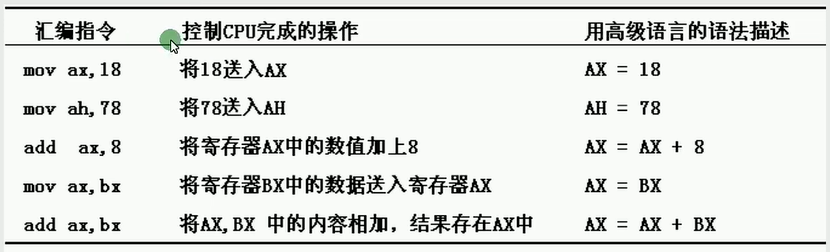
\includegraphics[scale=0.6]{汇编指令.png}
    \caption{汇编指令}
    \end{figure} 
\subsection{物理地址}
CPU访问内存单元时要给出内存单元的地址。

所有的内存单元构成的存储空间是一维的线性空间。

每一个内存单元在这个空间中都有唯一的地址,这个唯一的地址
称为物理地址。

事实:

8086有20位地址总线,可传送20位地址,寻址能力为1M

8086是16位结构的CPU
运算器一次最多可以处理16位数据,寄存器的最大宽度为16位

在8086内部处理的,传输,暂存的地址也是16位,选址能力也只有64kb

8086CPU的解决方法

用两个16位地址(段地址,偏移地址)合成一位20位的物理地址。

地址加法器合成物理地址的方法
物理地址 = 段地址 * 16 + 偏移地址
\begin{figure}[htbp]
    \centering
    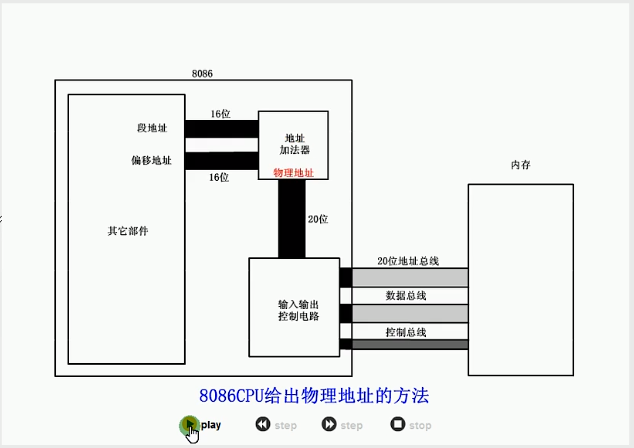
\includegraphics[scale=0.6]{物理地址.png}
    \caption{物理地址合成}
    \end{figure} 
本质含义:
CPU在访问内存时,用一个基础地址(段地址 * 16)和一个相对于基础地址的偏移地址
相加,给出内存单元的物理地址。
\subsection{分段形式管理内存}
\begin{figure}[htbp]
    \centering
    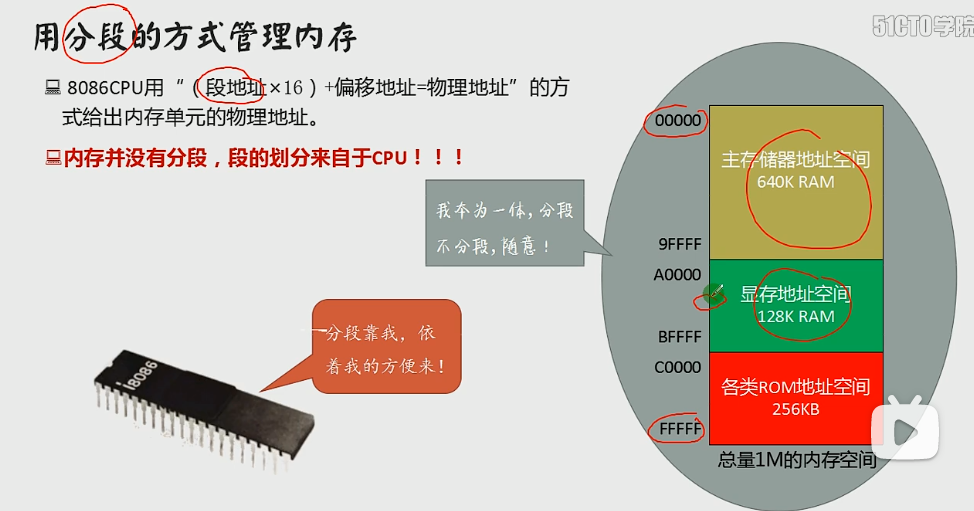
\includegraphics[scale=0.6]{分段形式管理内存.png}
    \caption{分段形式管理内存}
    \end{figure} 
\begin{figure}[htbp]
        \centering
        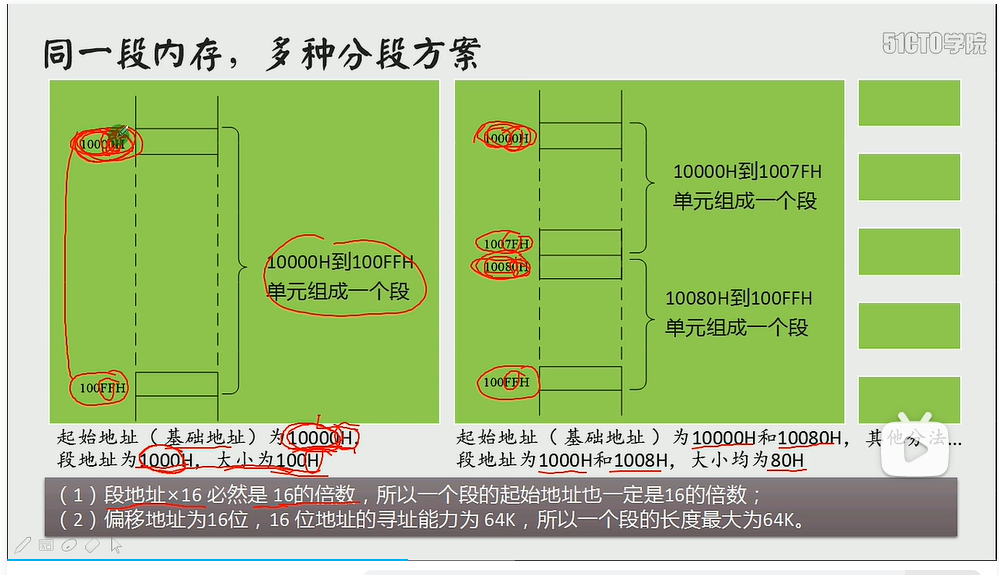
\includegraphics[scale=0.6]{分段方案.png}
        \caption{分段方案}
        \end{figure} 
补充:   寻址能力指的是CPU所能访问的内存的地址范围的大小,也就是说是内存的存储单元的大小
(这里自己是这么理解的,计算机存储了段地址,然后通过通过偏移地址来找到下一段,然后最大。。。。。。)
(每个存储单元可以存储1B)
\begin{figure}[htbp]
    \centering
    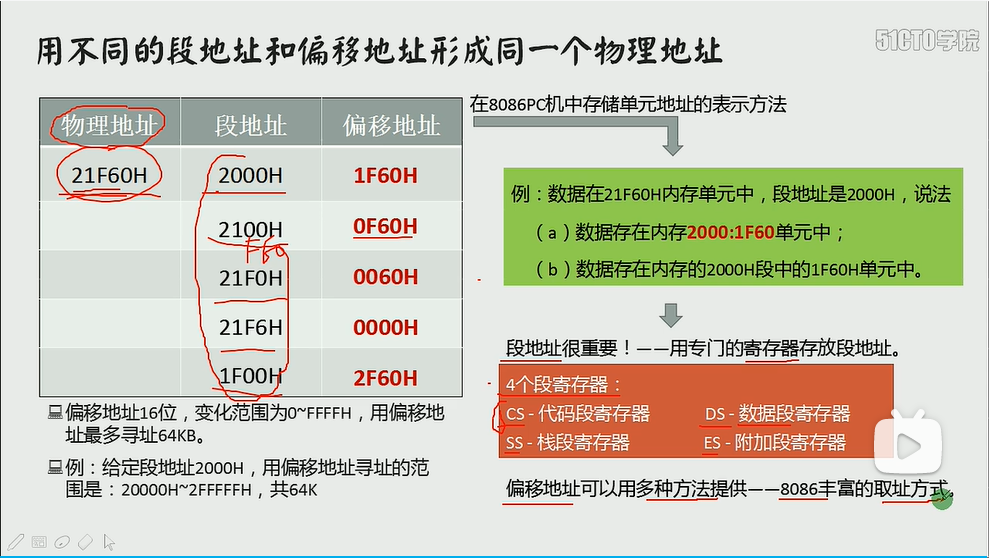
\includegraphics[scale=0.6]{不同形成同一.png}
    \caption{不同段形成同一物理地址}
    \end{figure} 
\subsection{DEBUG}
Debug 是dos系统中著名的调试程序,也可以运行在windows系统实模式下

\end{document}